% =====================================================================
%  Relatorio final — CCM-109 Deep Learning (UFABC)
%  Template SBC. Compilar no Overleaf: pdfLaTeX -> BibTeX -> pdfLaTeX x2
%
%  ATENCAO: o template original da SBC traz DUAS linhas de inputenc
%  (utf8 e latin1, nessa ordem). A ultima vence, e com latin1 todos os
%  acentos quebram. Aqui fica apenas utf8 — nao reinsira a linha latin1.
% =====================================================================
\documentclass[12pt]{article}

\usepackage{sbc-template}
\usepackage{graphicx,url}
\usepackage[utf8]{inputenc}
\usepackage[brazil]{babel}
\usepackage{booktabs}

\sloppy

\title{O jogador como token: um \emph{set Transformer} sobre \emph{freeze-frames}
       para estimativa de \emph{Expected Goals}}

\author{Vinícius Siqueira\inst{1}}

\address{Centro de Matemática, Computação e Cognição\\
  Universidade Federal do ABC (UFABC) -- Santo André, SP -- Brasil
  \email{vinicius.siqueira.data@gmail.com}
}

\begin{document}

\maketitle

\begin{abstract}
Expected Goals (xG) models estimate the probability that a shot results in a
goal. Classical models rely on hand-crafted interaction features such as
goalkeeper distance and the number of blockers. We ask whether a Transformer
that treats \textbf{each player as a token} learns this interaction geometry on
its own. Using 99{,}746 shots with StatsBomb freeze-frames, we compare a ladder
of models in which each rung adds exactly one capability, isolating the
contribution of pairwise attention. % TODO: fechar com o resultado quantitativo
\end{abstract}

\begin{resumo}
Modelos de \emph{Expected Goals} (xG) estimam a probabilidade de uma finalização
terminar em gol. Os modelos clássicos dependem de atributos de interação
desenhados à mão, como a distância do goleiro e o número de bloqueadores. Este
trabalho investiga se um Transformer que trata \textbf{cada jogador como um
token} aprende sozinho essa geometria de interação. Sobre 99.746 finalizações
com \emph{freeze-frames} da StatsBomb, comparamos uma escada de modelos em que
cada degrau acrescenta exatamente uma capacidade, isolando a contribuição da
atenção par a par. % TODO: fechar com o resultado quantitativo
\end{resumo}

% =====================================================================
\section{Descrição do Problema}

\emph{Expected Goals} (xG) é hoje a métrica central da análise de futebol
profissional: estima a probabilidade de uma finalização terminar em gol e
permite avaliar desempenho para além do placar, que é um sinal ruidoso e de
baixa frequência.

Os modelos clássicos de xG usam apenas atributos da própria finalização --
distância, ângulo de visão da baliza, parte do corpo. Quando incorporam os
demais jogadores, fazem-no por meio de atributos desenhados à mão: distância do
goleiro, número de defensores na linha do chute, pressão sobre o chutador. Cada
um desses atributos é uma hipótese humana sobre o que importa numa finalização.

Daí a pergunta que orienta este trabalho:

\begin{quote}
Um modelo que trata \textbf{cada jogador como um token} e usa \emph{self-attention}
aprende sozinho a geometria de interação que hoje exige engenharia manual de
atributos?
\end{quote}

A pergunta é interessante porque ambas as respostas são informativas. Se a
resposta for afirmativa, a engenharia manual de atributos de interação torna-se
dispensável. Se for negativa, isso indica que a informação relevante está
\emph{por jogador} e não \emph{entre jogadores} -- um resultado que contraria a
intuição de que futebol é um jogo de interações.

\subsection{Definição formal}

Cada finalização é um par (cena, desfecho). A cena é um \textbf{conjunto} de até
22 jogadores, cada um descrito por um vetor de atributos geométricos; o desfecho
é binário. O objetivo é aprender uma função que mapeia o conjunto em uma
probabilidade no intervalo $[0,1]$.

A propriedade que define o problema é a \textbf{invariância à permutação}: a
ordem em que os jogadores são listados não carrega informação e, portanto,
embaralhá-la não pode alterar a previsão. Isso distingue a tarefa de problemas
sequenciais e justifica a ausência de \emph{positional encoding}
(Seção~\ref{sec:arq}).

% =====================================================================
\section{Abordagem}

\subsection{Dados}

Utilizamos a StatsBomb Open Data, base pública sob licença de uso não comercial
com atribuição. Para cada finalização, a base registra o \emph{freeze-frame}: as
coordenadas $(x,y)$ de todos os jogadores visíveis no instante do chute, com
seus papéis (companheiro, adversário, goleiro) e o desfecho do lance. Após
excluir pênaltis e lances sem \emph{freeze-frame}, restam 99.746 finalizações de
3.961 partidas em 80 competições-temporada, com taxa de gol de 10,26\%.

\subsubsection*{Limitações declaradas dos dados}

\begin{itemize}
  \item O \emph{freeze-frame} fornece \textbf{posição, mas não velocidade nem
        direção}. Um defensor parado e outro em corrida de recuperação são
        indistinguíveis para o modelo.
  \item \textbf{30,7\% das finalizações vêm de competições femininas} e cerca de
        37\% de apenas quatro temporadas 2015/16 de ligas europeias. As taxas de
        gol dos dois grupos são praticamente iguais (10,4\% contra 10,2\%), o que
        sustenta tratá-los conjuntamente, mas a decisão é declarada e não
        silenciosa.
  \item A média é de \textbf{13,1 jogadores visíveis por cena}, não 22. O
        mascaramento das posições vazias é, portanto, o caso comum e não a
        exceção.
\end{itemize}

\subsection{Representação: o jogador como token}

Cada cena é convertida em um conjunto de até 22 tokens (o chutador e os jogadores
do \emph{freeze-frame}), cada um com 14 atributos: geometria absoluta, geometria
\textbf{relativa ao chutador e à linha do chute} (projeção sobre a linha,
distância perpendicular, presença no triângulo formado com os postes) e
indicadores de papel.

A escolha dos atributos relativos é deliberada: eles informam a cada token sua
própria relação com a finalização, \textbf{sem} codificar relações par a par
entre jogadores. Isso mantém a ablação honesta, pois o que separa o Deep Sets do
Transformer continua sendo apenas a atenção.

\subsection{Arquitetura}\label{sec:arq}

\emph{Encoder} Transformer compacto: 2 camadas, 4 cabeças, dimensão 48, token
\texttt{[CLS]}, \textbf{sem \emph{positional encoding}} e com máscara de
\emph{padding} nas posições sem jogador. Saída sigmoide. Implementação em
PyTorch.

% TODO: figura do diagrama da arquitetura (cena -> tokens -> encoder -> xG)

\subsection{Protocolo experimental}

\textbf{Escada de \emph{baselines}.} Cada degrau acrescenta exatamente uma
capacidade, de modo que a diferença entre degraus atribui o mérito a um
componente específico:

\begin{table}[ht]
\centering
\caption{Escada de modelos. Cada degrau acrescenta uma única capacidade.}
\label{tab:escada}
\begin{tabular}{@{}lll@{}}
\toprule
 & Modelo & O que acrescenta \\
\midrule
B1 & Regressão logística: distância, ângulo, cabeceio & o xG ``de livro'' \\
B2 & B1 + atributos manuais de interação & interação \textbf{feita à mão} \\
DS & Deep Sets sobre os tokens & informação por jogador \\
TF & Transformer sobre os mesmos tokens & interação \textbf{aprendida} \\
\bottomrule
\end{tabular}
\end{table}

A comparação decisiva é \textbf{TF contra DS}: ambos recebem exatamente os mesmos
tokens, e apenas o Transformer pode comparar jogadores entre si.

\textbf{Divisão dos dados por partida} (70/15/15). Finalizações da mesma partida
compartilham time, adversário e contexto tático; separá-las entre treino e teste
inflaria as métricas por vazamento.

\textbf{Métricas.} AUC (ordenação), \emph{log loss}, \textbf{Brier score} e
\textbf{curva de calibração} (qualidade da probabilidade). Como xG é uma
probabilidade e não um \emph{ranking}, o Brier é a métrica de decisão; a AUC o
acompanha para distinguir ``ordena bem'' de ``acerta o valor''.

\textbf{Significância.} As diferenças entre modelos são avaliadas por
\emph{bootstrap} pareado \textbf{agrupado por partida}: reamostram-se partidas,
não finalizações, porque chutes do mesmo jogo são correlacionados e reamostrá-los
individualmente produziria intervalos de confiança estreitos demais.

% =====================================================================
\section{Resultados}

% TODO: esta secao esta parcial. Apenas o EXP-000 foi executado.

\subsection{Escada de \emph{baselines}}

\begin{table}[ht]
\centering
\caption{Desempenho no conjunto de teste (14.935 finalizações), divisão por
partida. Modelos neurais: média de 2 sementes.}
\label{tab:resultados}
\begin{tabular}{@{}lrrr@{}}
\toprule
Modelo & AUC & \emph{Log loss} & Ganho em AUC \\
\midrule
B1 & 0,7653 & 0,2887 & --- \\
B2 & 0,7961 & 0,2739 & +0,0308 \\
DS & 0,8144 & 0,2659 & +0,0183 \\
TF & 0,8158 & 0,2650 & +0,0014 \\
\bottomrule
\end{tabular}
\end{table}

\begin{figure}[ht]
\centering
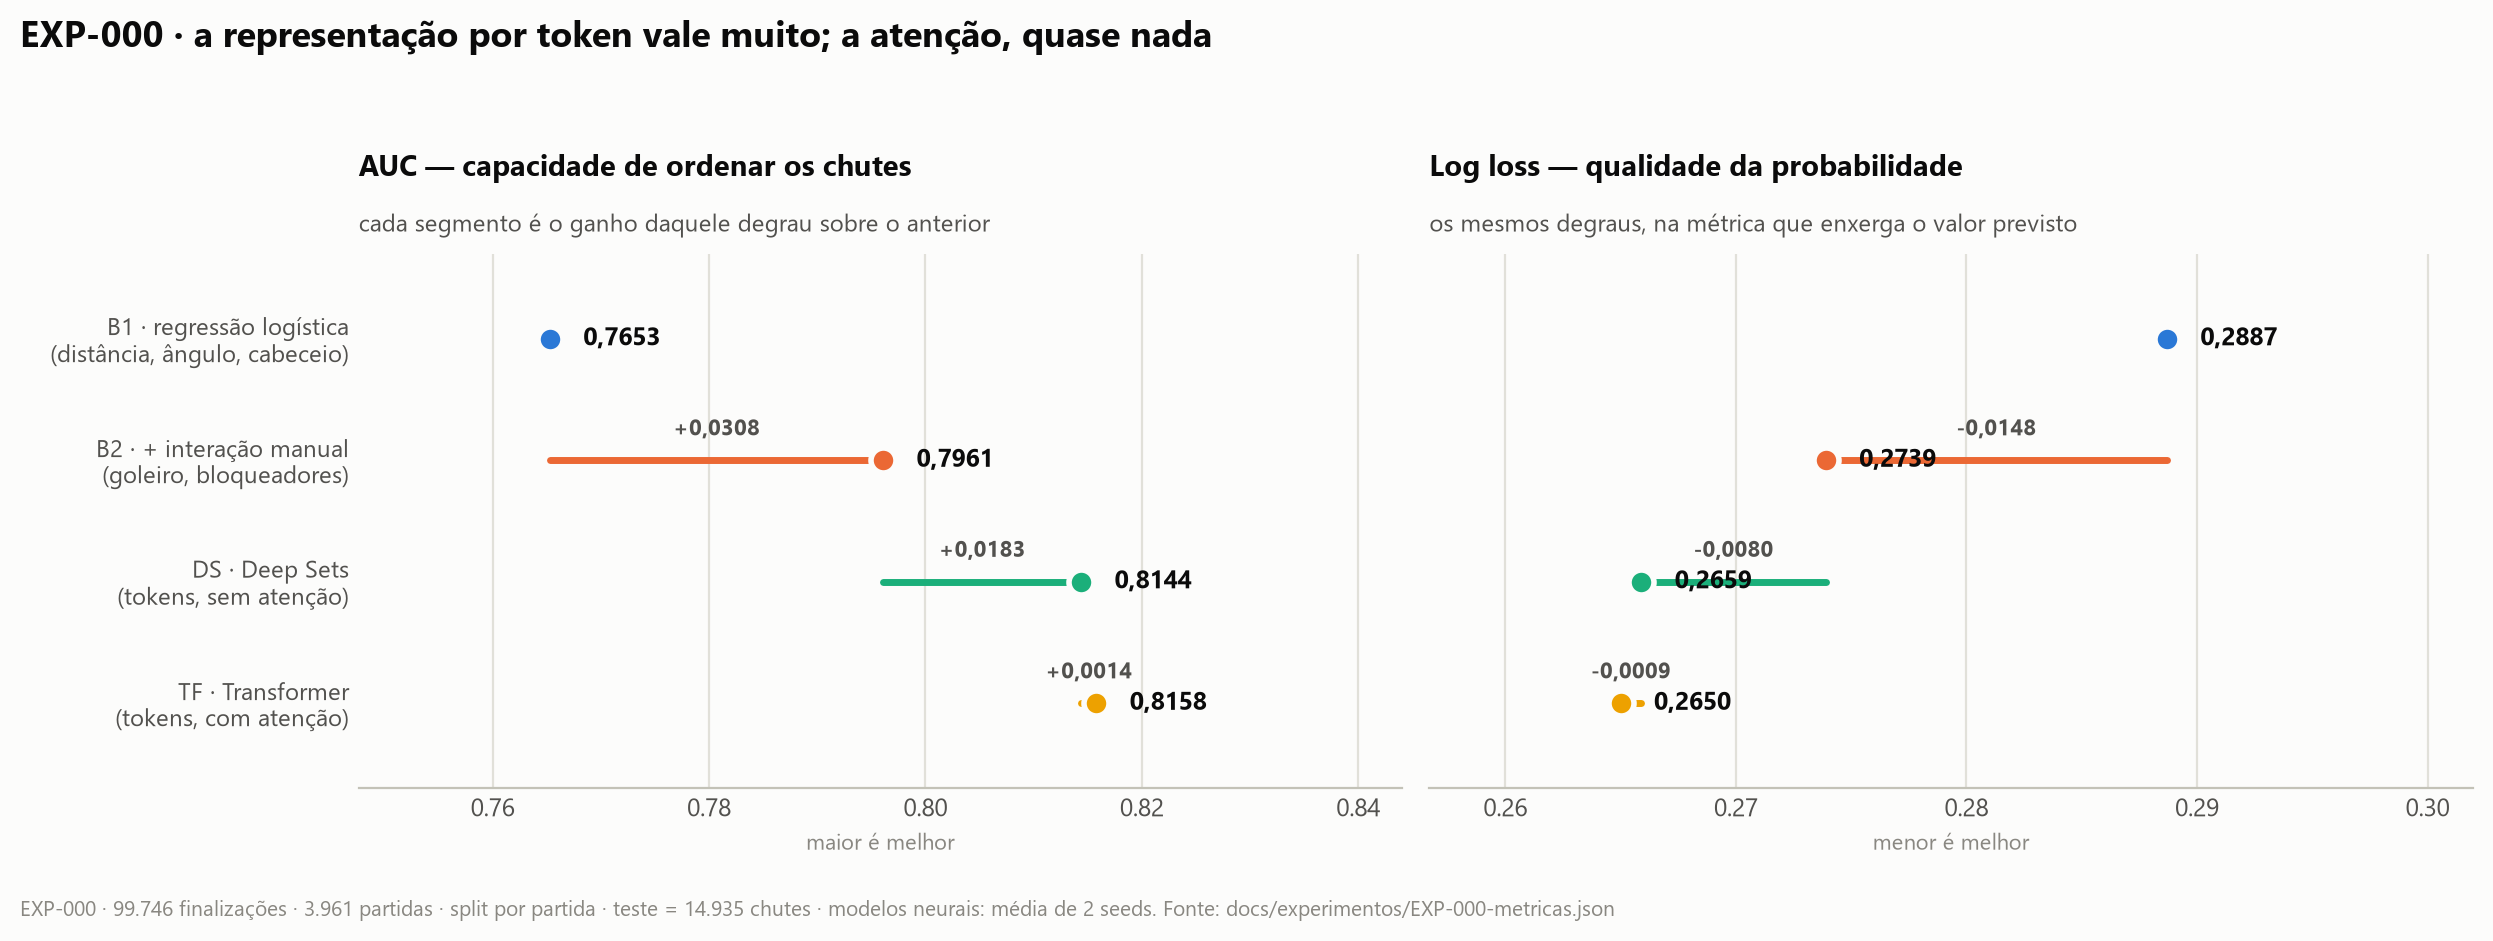
\includegraphics[width=\textwidth]{figuras/EXP-000-escada.png}
\caption{Ganho de cada degrau da escada. Cada segmento representa o incremento
sobre o degrau anterior.}
\label{fig:escada}
\end{figure}

Dois achados. Primeiro, a representação por token tem valor claro: o salto de B2
para Deep Sets (+0,0183 de AUC) mostra que fornecer a cena inteira ao modelo
supera resumi-la em atributos manuais. Segundo, e mais relevante para a pergunta
do trabalho, \textbf{a atenção acrescenta pouco} sobre o Deep Sets: +0,0014 de
AUC, valor da mesma ordem do desvio entre sementes.

% TODO: 3.2 calibracao (EXP-000)
% TODO: 3.3 TF vs DS com 5 sementes e bootstrap pareado (EXP-004)
% TODO: 3.4 mapas de atencao (EXP-005)
% TODO: 3.5 estudo de caso: Eurocopa 2024

% =====================================================================
\section{Lições Aprendidas}

\subsection{O que funcionou}

\textbf{Escalar os dados resolveu o que aparentava ser um problema de
arquitetura.} Na prova de conceito, com 6.347 finalizações, os modelos neurais
alcançavam AUC de aproximadamente 0,71 -- \emph{abaixo} do \emph{baseline} com
atributos manuais (0,736). Com 99.746 finalizações, ambos os modelos neurais
superam esse \emph{baseline} com folga. A conclusão precipitada de que ``a
arquitetura não serve'' teria sido incorreta.

% TODO: 4.2 o que nao funcionou (tentativas T1-T4)
% TODO: 4.3 o que eu faria diferente

% =====================================================================
\section*{Disponibilidade do código}

Todo o código, a documentação de decisões e o registro de experimentos estão em
\url{https://github.com/vinisique/xg-set-transformer}.

\bibliographystyle{sbc}
\bibliography{referencias}

\end{document}
